\documentclass[ignorenonframetext,red]{beamer}

\usepackage{ucs}
\usepackage{mathpartir}
\usepackage{amsfonts,amsmath}
\usepackage{stmaryrd}
\usepackage[utf8x]{inputenc}
\usepackage[protrusion=true,expansion=true]{microtype}
\usepackage{setspace}
\usepackage{graphicx}
\usepackage{natbib}
\usepackage{listings}

\usepackage{../../macros}

\date{\\[1em] June 2011 \\[1em]
\scriptsize INRIA -- Gallium}

\title{A logical framework for incremental type-checking}

\author[Matthias Puech \& Yann Régis-Gianas] {
  Matthias Puech\inst{1,2} \and Yann Régis-Gianas\inst{2}
}

\institute {
  \inst 1 {Dept. of Computer Science, University of Bologna} \and
  \inst 2 {University Paris 7, CNRS, and INRIA, PPS, team ${\pi}r^2$}
}

\setbeamertemplate{footline}[frame number]
\setbeamertemplate{navigation symbols}{}
\setbeamertemplate{itemize item}[circle]

\usefonttheme{serif}

\AtBeginSection[]
{\begin{frame}<beamer>{Menu}
    \tableofcontents[currentsection]
  \end{frame}
}
\lstset{
  language=[Objective]Caml,
  basicstyle=\sf,
  columns=flexible,
  literate={->}{{$\to$ }}1 {*}{$\times$ }1 {>=}{{$\geq$}}1
  {<>}{{$\neq$}}1 {'a}{{$\alpha$}}1 {'b}{{$\beta$}}1 {'c}{{$\gamma$}}1
}

\newcommand\sz[1]{\hsubst{#1}\mmmv\mval}

\begin{document}

\frame\titlepage


\begin{frame}{A paradoxical situation}  
  \begin{block}{Observation}
    We have powerful tools to mechanize the metatheory of (proof) languages
  \end{block}
  \pause
  \begin{block}{\ldots\ And yet,}
    Workflow of programming and formal mathematics is still largely inspired by legacy
    software development (\textsf{emacs}, \textsf{make}, \textsf{svn},
    \textsf{diff}s\ldots)
  \end{block}
  \vspace{0.6em}
  \pause
  \begin{center}
    {\large \it Isn't it time to make these tools metatheory-aware?}
  \end{center}
\end{frame}

\begin{frame}{Incrementality in programming {\it \&} proof languages}
\vspace{1em}
  {\Huge Q {\Large :}} \parbox{0.8\textwidth}{Do you spend more time
    \emph{writing} code or \emph{editing} code?} \\[2em]

Today, we use:
  \begin{itemize}
  \item separate compilation
  \item dependency management
  \item version control on the scripts
  \item interactive toplevel with global rollback (\textsf{Coq})
  \end{itemize}
  \pause
  \begin{center}
    \large\ldots\ ad-hoc tools, code duplication, hacks\ldots
  \end{center}
  \footnotesize
  \begin{examples}\vspace{-0.5em}
    \begin{itemize}
    \item \texttt{diff}'s language-specific options, lines of context\ldots
    \item \texttt{git}'s merge heuristics
    \item \texttt{ocamldep} \emph{vs.} \texttt{ocaml} module system
    \item \texttt{coqtop}'s rigidity
    \end{itemize}
  \end{examples}
\end{frame}

\begin{frame}{In an ideal world\ldots}
  \begin{itemize}
  \item Edition should be incrementally communicated to the tool
  \item The impact of changes visible “in real time”
  \item No need for separate compilation, dependency management\ldots
  \end{itemize}
  \pause
  \vspace{2em}
  \begin{center}
    {\large \it Types are good witnesses of this impact}
  \end{center}
  \vspace{1em}
  \pause
  \begin{block}{Applications}
    \vspace{-0.5em}
    \footnotesize
    \begin{itemize}
    \item non-(linear$|$batch) user interaction
    \item typed version control systems
    \item type-directed programming
    \item tactic languages
    \end{itemize}
  \end{block}
\end{frame}

\begin{frame}{In this talk, we focus on\ldots}
  \ldots\ building a procedure to type-check \emph{local changes}

  \begin{itemize}
  \item What data structure for storing type derivations?
  \item What language for expressing changes?
  \end{itemize}
\end{frame}

\begin{frame}{Menu}
  \tableofcontents
\end{frame}

\section{The big picture}

\begin{frame}{The big picture}
  \begin{center}
    \only<1-2>{\fbox{\parbox{20em}{\only<2>\alert{version
            management}\\[1em]%
          \fbox{\parbox{18em}{script files\\[1em]%
              \fbox{\parbox{17em}{parsing\\[1em]%
                  \fbox{\parbox{14em}{type-checking\\} }}}}}}}}%
    \only<3>{\fbox{\parbox{20em}{script files\\[1em]%
          \fbox{\parbox{18em}{\alert{version management}\\[1em]%
              \fbox{\parbox{17em}{parsing\\[1em]%
                  \fbox{\parbox{14em}{type-checking\\} }}}}}}}}%
    \only<4-6>{\fbox{\parbox{20em}{
          \begin{overlayarea}{20em}{2em}
            \alt<-5>{script files}{user interaction}
          \end{overlayarea}%
          \fbox{\parbox{18em}{parsing\\[1em]%
              \fbox{\parbox{17em}{\alert{version management}\\[1em]%
                  \uncover<4-6>{\fbox{\parbox{14.5em}{type-checking\\}}}}}}}}}}%
    \only<7->{\fbox{\parbox{20em}{
          \begin{overlayarea}{20em}{2em}
            user interaction
          \end{overlayarea}%
          \fbox{\parbox{18em}{parsing\\[1em]%
              \fbox{\parbox{17em}{\only<8->{incremental }type-checking\\[1em]%
                  \fbox{\parbox{14.5em}{\alert{version management}\\}}}}}}}}}%
  \end{center}
  \begin{itemize}
  \item<4-> AST representation
  \item<7-> Typing annotations
  \end{itemize}
\end{frame}

\subsection{Incremental type-checking}

\begin{frame}[fragile]{\gray{A logical framework for incremental}
    type-checking}
  Yes, we're speaking about (any) typed language.
  \begin{block}{A type-checker}
    \begin{lstlisting}
      val check : env -> term -> types -> bool
    \end{lstlisting}
    \begin{itemize}
    \item builds and checks the derivation (on the stack)
    \item conscientiously discards it
    \end{itemize}
  \end{block}
  % \pause
  % \def\envbarb{A\to B, B\to C, A\vdash}
  
  % \begin{overlayarea}{\textwidth}{7em}
  %   \alt<-2>{
  %     \[ \tiny
  %     \def\impi{{\tiny$\to_i$}}
  %     \def\impe{{\tiny$\to_e$}}
  %     \def\ax{{\tiny$Ax$}}
  %     \infer*[left=\impi]{
  %       \infer*[left=\impi]{
  %         \infer*[left=\impi]{
  %           \infer*[left=\impe]{
  %             \infer*[right=\ax,leftskip=5em]{ }{\envbarb B\to C}\\
  %             \infer*[right=\impe,rightskip=5em]{
  %               \infer*[right=\ax]{ }{\envbarb A\to B}\\
  %               \infer*[right=\ax]{ }{\envbarb A}
  %             }{\envbarb B}
  %           }{\envbarb C}
  %         }{A\to B, B\to C\vdash A\to C}
  %       }{A\to B\vdash (B\to C)\to A\to C}
  %     }{\vdash (A\to B)\to(B\to C)\to A\to C}
  %     \]
  %   }{
  %     \begin{center}
  %       \vspace{3em}
  %       \large \textsf{\textbf{true}}
  %     \end{center}
  %   }
  % \end{overlayarea}
  % \pause  
\end{frame}

\begin{frame}{\gray{A logical framework for} incremental
    \gray{type-checking}}
    \begin{description}
    \item[Goal] Type-check a large derivation taking advantage of the
      knowledge from type-checking previous versions
    \item[Idea] Remember all derivations!
    \end{description}
    \pause \inXLF
    \begin{overlayarea}\textwidth{12em}
      \begin{onlyenv}<-3>
        \begin{block}{More precisely}
          Given a well-typed $\mr : repository$ and a $\delta : delta$
          and $$\mathsf{apply} : repository \to delta \to derivation\ ,$$an
          incremental type-checker $$\mathsf{tc} : repository \to
          delta \to \alt<-2>{bool}{repository\ option} $$ decides if
          $\mathsf{apply}(\delta,\mr)$ is
          well-typed in $O(|\delta|)$. \\
          {\hfill\scriptsize (and not
            $O(|\mathsf{apply}(\delta,\mr)|)$)}
        \end{block}
      \end{onlyenv}
      \begin{onlyenv}<4->
        \textbf{from}\\
        {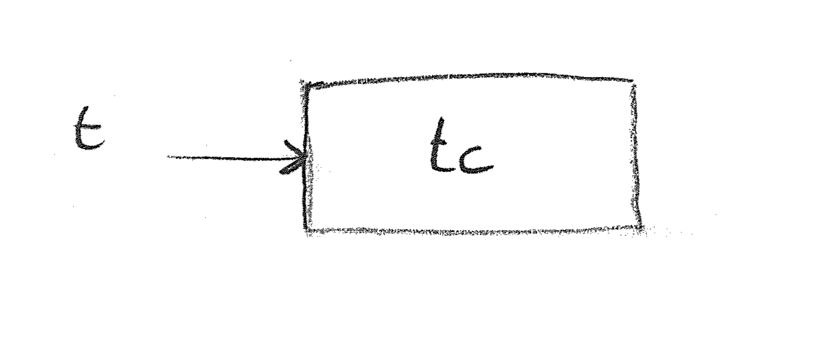
\includegraphics[width=0.5\textwidth]{images/tc-classic.png}} \\
        \textbf{to}\\
        {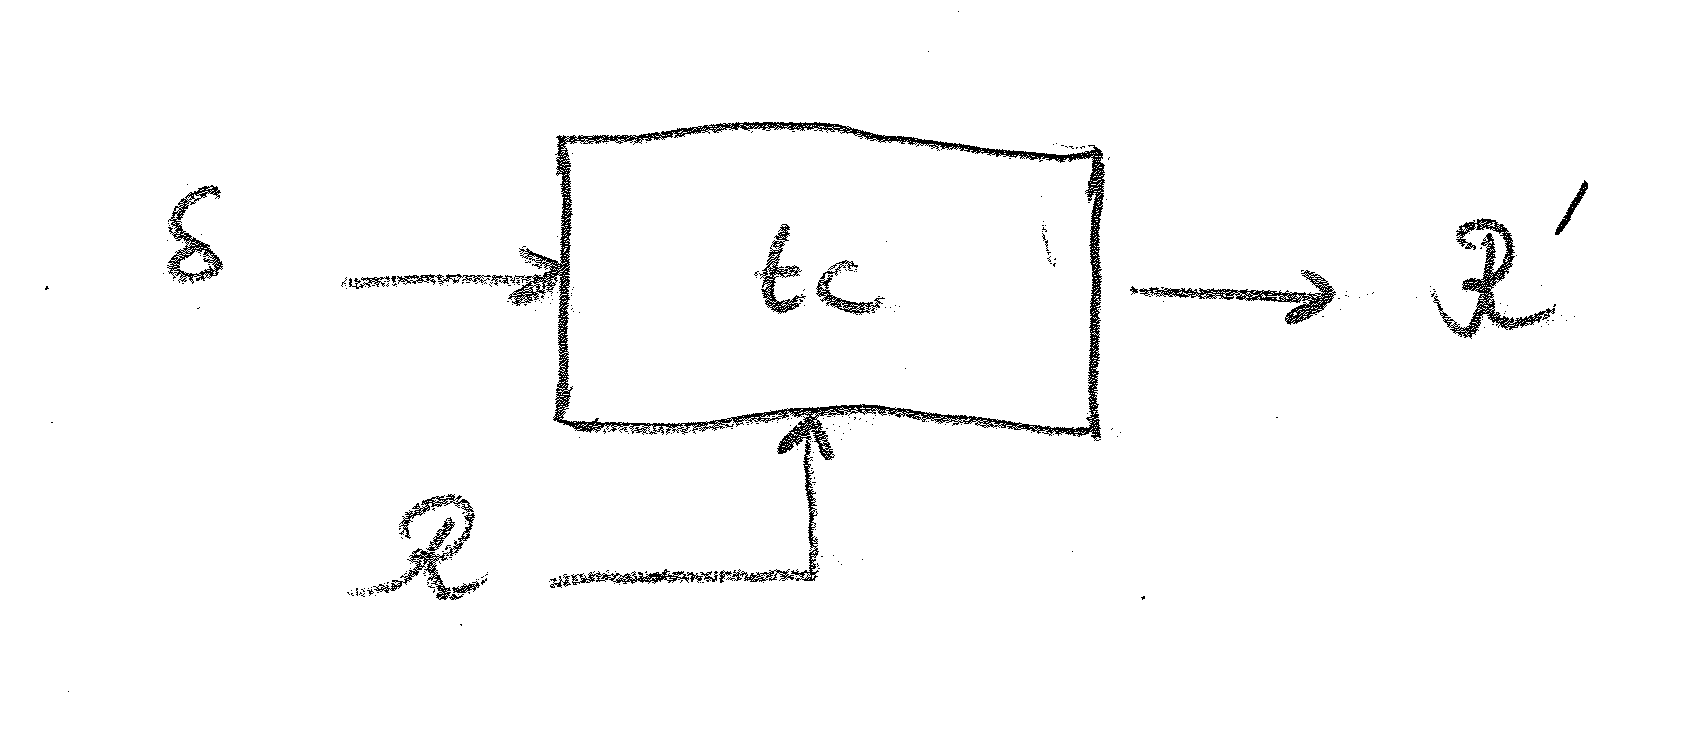
\includegraphics[width=0.5\textwidth]{images/tc-delta1.png}} \\
      \end{onlyenv}
    \end{overlayarea}
\end{frame}

\subsection{Why not memoization?}

\begin{frame}[fragile]{Memoization maybe?}
  \begin{onlyenv}<1>
    \vspace{4em}
\begin{lstlisting}
let rec check env t a = 
  match t with
  | ... -> ... false
  | ... -> ... true

and infer env t =
  match t with 
  | ... -> ... None
  | ... -> ... Some a
\end{lstlisting}
  \end{onlyenv}
  \begin{onlyenv}<2>
    \vspace{3em}
\begin{lstlisting}
let table = ref ([] : environ * term * types) in
let rec check env t a = 
  if List.mem (env,t,a) !table then true else
    match t with
    | ... -> ... false
    | ... -> ... table := (env,t,a)::!table; true
and infer env t =
  try List.assoc (env,t) !table with Not_found ->
    match t with 
    | ... -> ... None
    | ... -> ... table := (env,t,a)::!table; Some a
\end{lstlisting}
  \end{onlyenv}
  \pause\pause
  \begin{block}{Syntactically}
    \begin{enumerate}
    \item[\itplus] lightweight, efficient implementation
      \pause
    \item[\itplus] $repository = \mathsf{table}$, $delta =
      \mathsf{t}$
      \pause
    \item [\itminus] syntactic comparison (no quotient on judgements) \\
    {\footnotesize What if I want \emph{e.g.} weakening or
      permutation to be taken into account?}
    \end{enumerate}
  \end{block}
  \pause
  \vspace{-1em}
  \begin{block}{Semantically}
    \begin{enumerate}
    \item[\itminus] external to the type system (meta-cut) \\
      {\footnotesize What does it mean logically?
        \begin{mathpar}
          \tiny
          \infer {J\in \Gamma} {\Gamma\vdash \jwf J\To \Gamma} \and
          \infer {\Gamma_1\vdash \jwf{J_1} \To \Gamma_2\\\ldots\\
            \Gamma_{n-1}[J_{n-1}]\vdash \jwf{J_n}\To \Gamma_n}
          {\Gamma_1\vdash \jwf J\To \Gamma_n[J_n][J]}
        \end{mathpar}
      }
      \pause
    \item[\itminus] imperative (introduces a dissymmetry)
    \end{enumerate}
  \end{block}
  \pause
  {\footnotesize Mixes two goals:} {\large \it derivation synthesis}
  {\footnotesize \&} {\large \it object reuse}
\end{frame}

\section{Our approach}

\subsection{Two-passes type-checking}

\begin{frame}{Two-passes type-checking}
  \begin{center}
    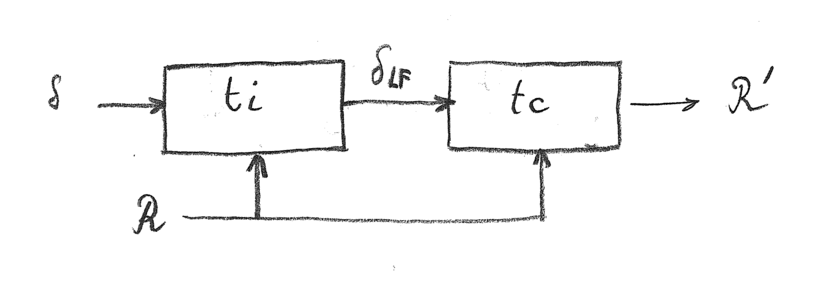
\includegraphics[width=0.7\textwidth]{images/tc-delta2.png}
  \end{center}
  \begin{description}
    \item[\textsf{ti}] = type inference = derivation delta synthesis
    \item[\textsf{tc}] = type checking = derivation delta checking
    \item[$\delta$] = program delta
    \item[$\delta_{LF}$] = derivation delta
    \item[$\mr$] = repository of derivations
  \end{description}
  \vspace{1em}
  \pause
  \emph{Shift of trust:} \textsf{ti} (complex, ad-hoc algorithm) $\to$ \textsf{tc}
  (simple, generic kernel)
\end{frame}

\subsection{The data-oriented way}

\begin{frame}{A popular storage model for directories}
  \begin{onlyenv}<1-7>
    \begin{center}
      \only<+>{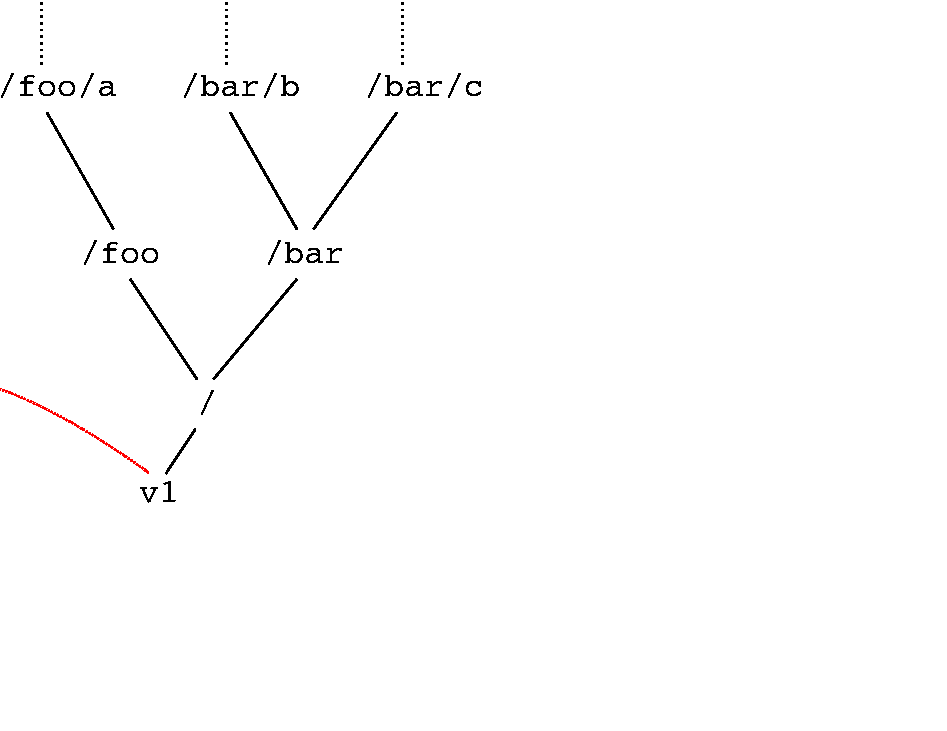
\includegraphics[width=0.85\textwidth]{images/git1.pdf}}%
      \only<+>{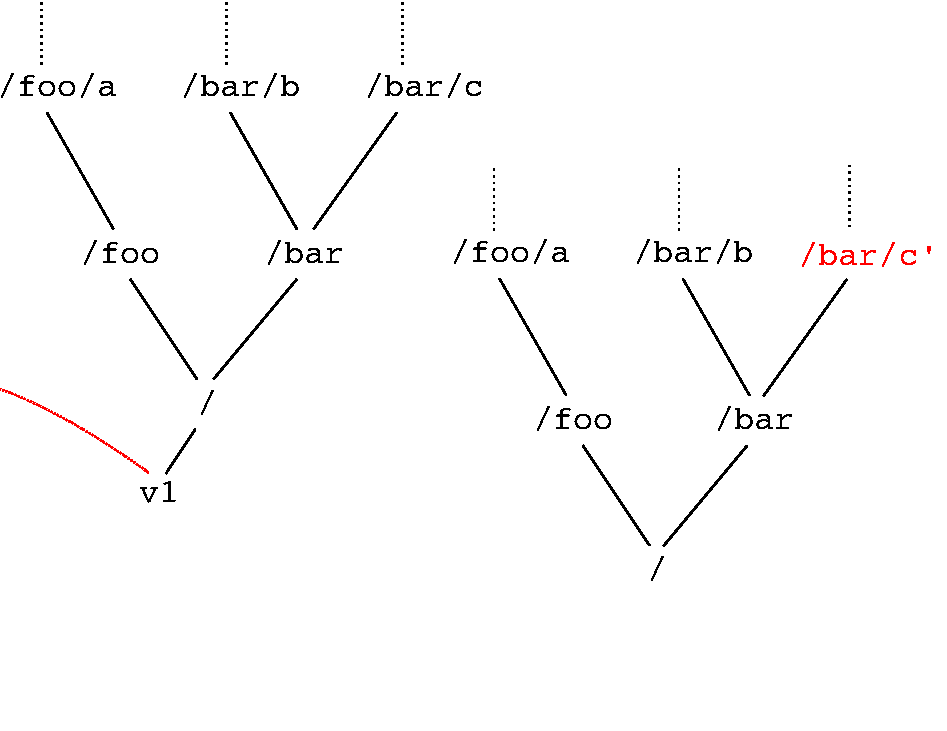
\includegraphics[width=0.85\textwidth]{images/git2.pdf}}%
      \only<+>{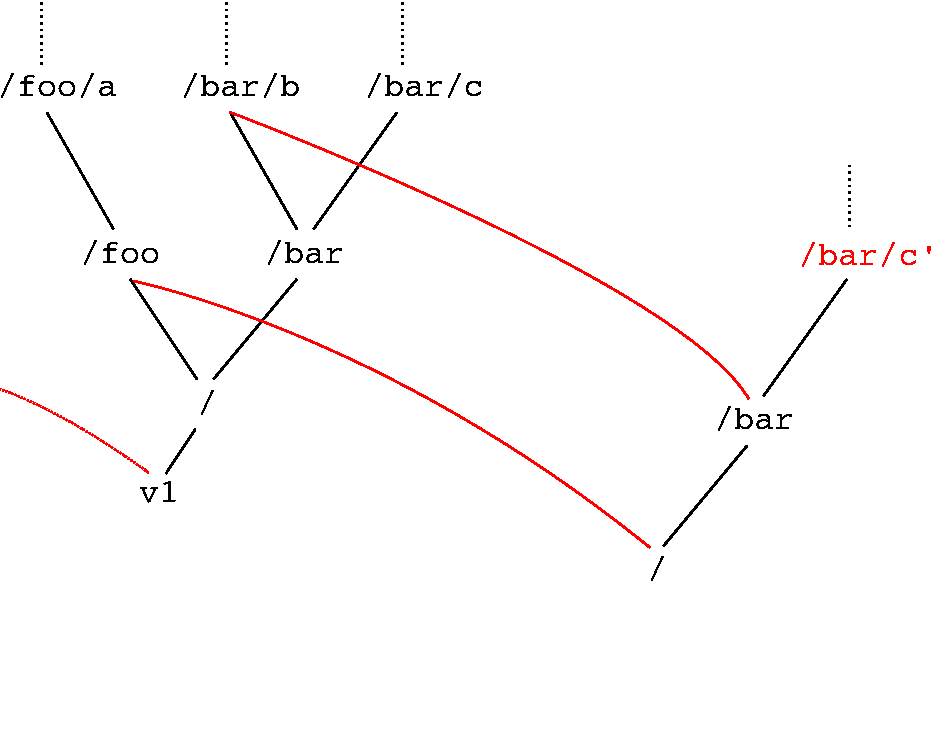
\includegraphics[width=0.85\textwidth]{images/git3.pdf}}%
      \only<+>{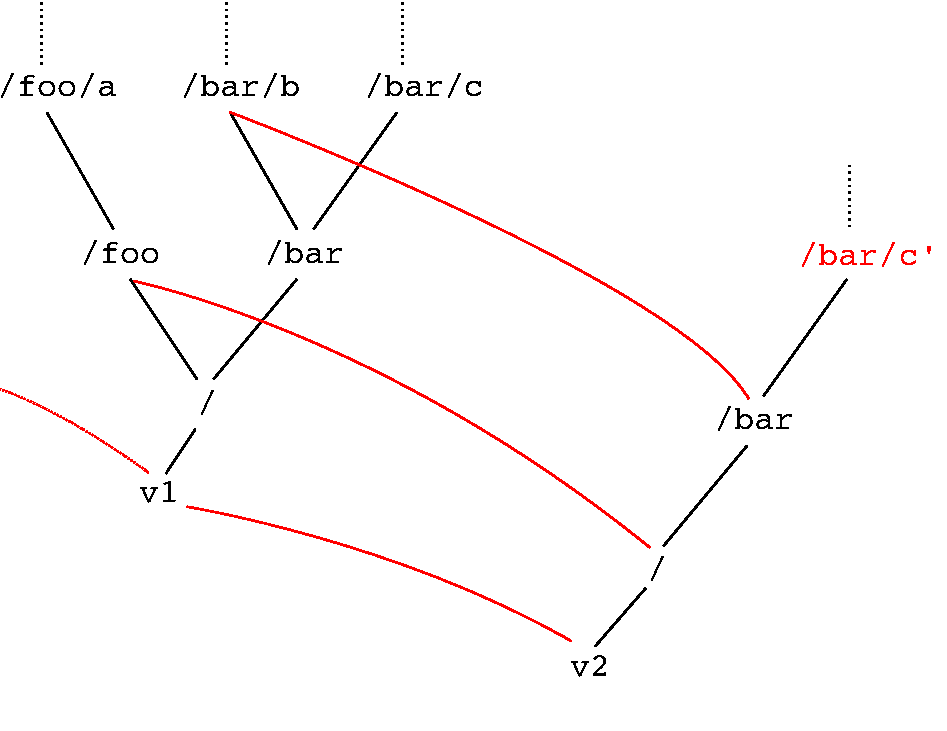
\includegraphics[width=0.85\textwidth]{images/git4.pdf}}%
      \only<+>{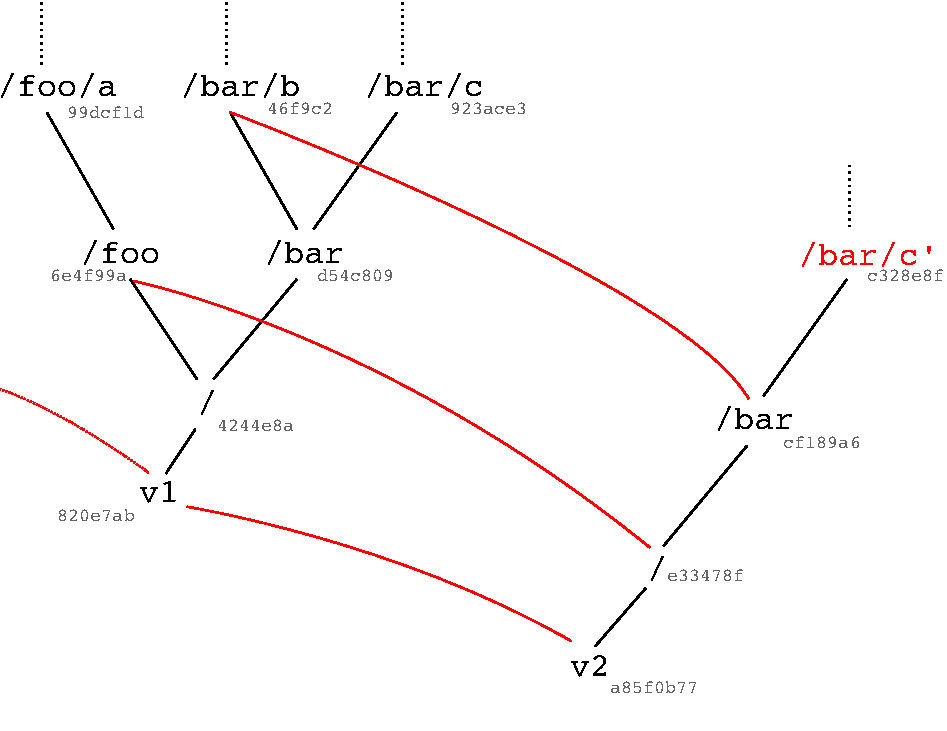
\includegraphics[width=0.85\textwidth]{images/git5.pdf}}%
      \only<+>{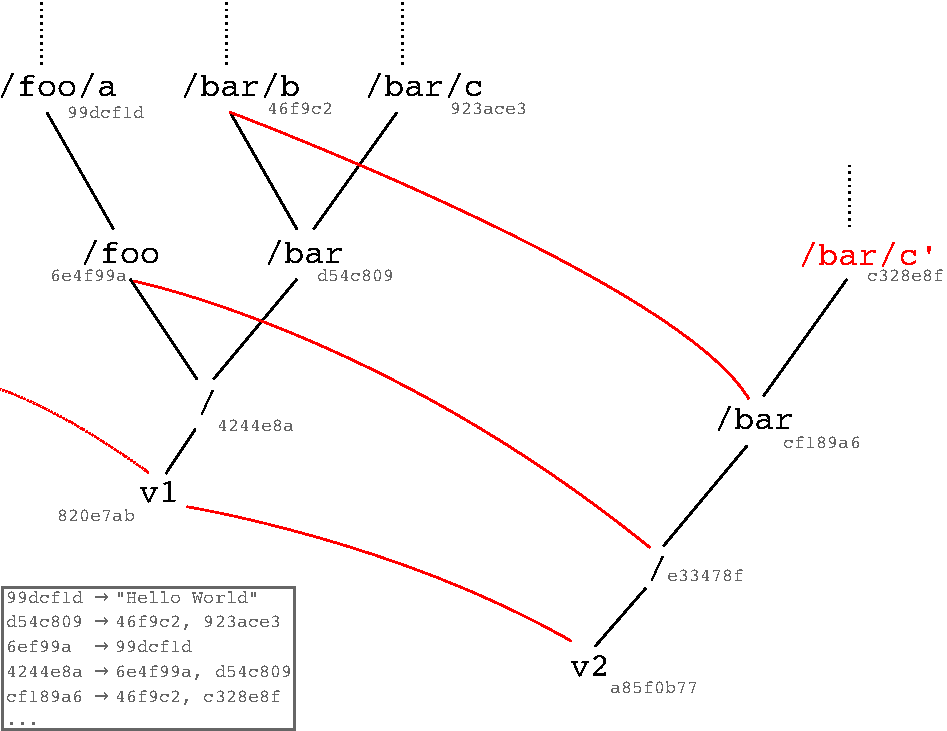
\includegraphics[width=0.85\textwidth]{images/git6.pdf}}%
      \only<+>{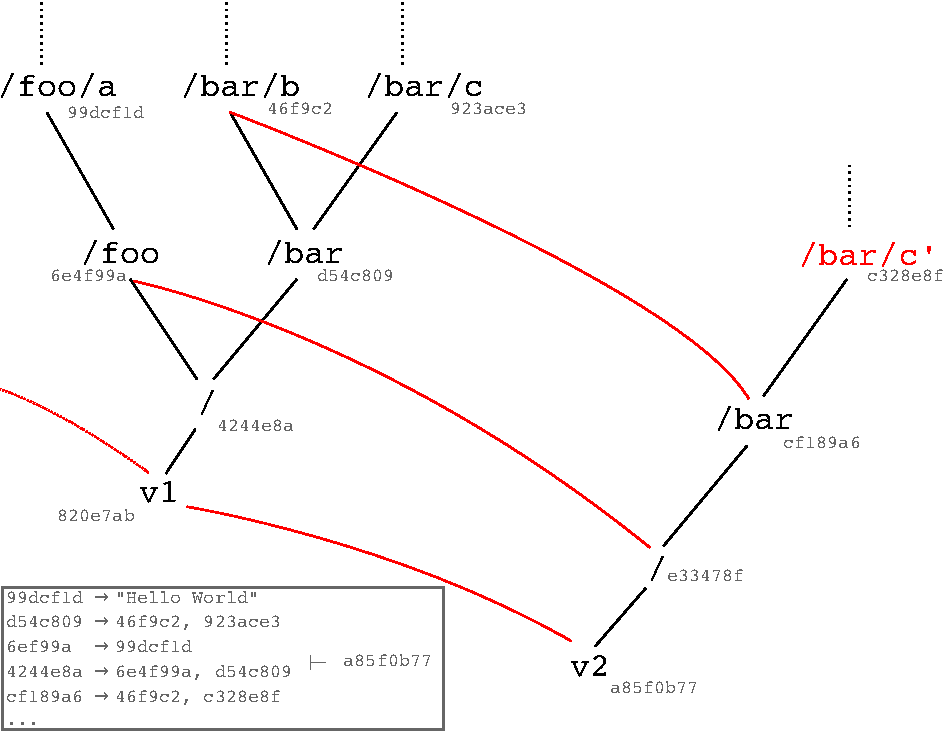
\includegraphics[width=0.85\textwidth]{images/git7.pdf}}%
    \end{center}
  \end{onlyenv}
  \begin{onlyenv}<8->
    The repository $\mr$ is a pair $(\Delta, x)$:
    \[ \Delta : x \mapsto (\mathsf{Commit}\ (x\times y) \gor \mathsf{Tree}\ \vec x
    \gor \mathsf{Blob}\ string)\]
    \begin{overlayarea}{\textwidth}{12em}
      \begin{onlyenv}<8>
        \begin{block}{Operations}
          \begin{description}
          \item[\texttt{commit $\delta$}]
            \begin{itemize}
            \item extend the database with \textsf{Tree}/\textsf{Blob}
              objects
            \item add a \textsf{Commit} object
            \item update head
            \end{itemize}
          \item[\texttt{checkout $v$}]
            \begin{itemize}
            \item follow $v$ all the way to the \textsf{Blob}s
            \end{itemize}
          \item[\texttt{diff $v_1$ $v_2$}]
            \begin{itemize}
            \item follow simultaneously $v_1$ and $v_2$
            \item if object names are equal, stop (content is equal)
            \item otherwise continue
            \end{itemize}
          \item[\dots]
          \end{description}
        \end{block}
      \end{onlyenv}
      \begin{onlyenv}<9->
        \begin{block}{Invariants}
          \begin{itemize}
          \item $\Delta$ forms a DAG
          \item if $(x, \mathsf{Commit}\ (y,z)) \in\Delta$ then
            \begin{itemize}
            \item $(y, \mathsf{Tree}\ t)\in\Delta$
            \item $(z, \mathsf{Commit}\ (t,v))\in\Delta$
            \end{itemize}
          \item if $(x, \mathsf{Tree}(\vec y))\in\Delta$ then \\
            for all $y_i$, either $(y_i, \mathsf{Tree}(\vec z))$ or
            $(y_i, \mathsf{Blob}(s))\in\Delta$
          \end{itemize}
        \end{block}
    \begin{onlyenv}<10>
      \begin{center}
        {\Large Let's do the same with \emph{proofs}}
      \end{center}
    \end{onlyenv}
      \end{onlyenv}
    \end{overlayarea}
  \end{onlyenv}
\end{frame}

\begin{frame}[fragile]{A \emph{typed} repository of proofs}
  \begin{center}
    \only<+>{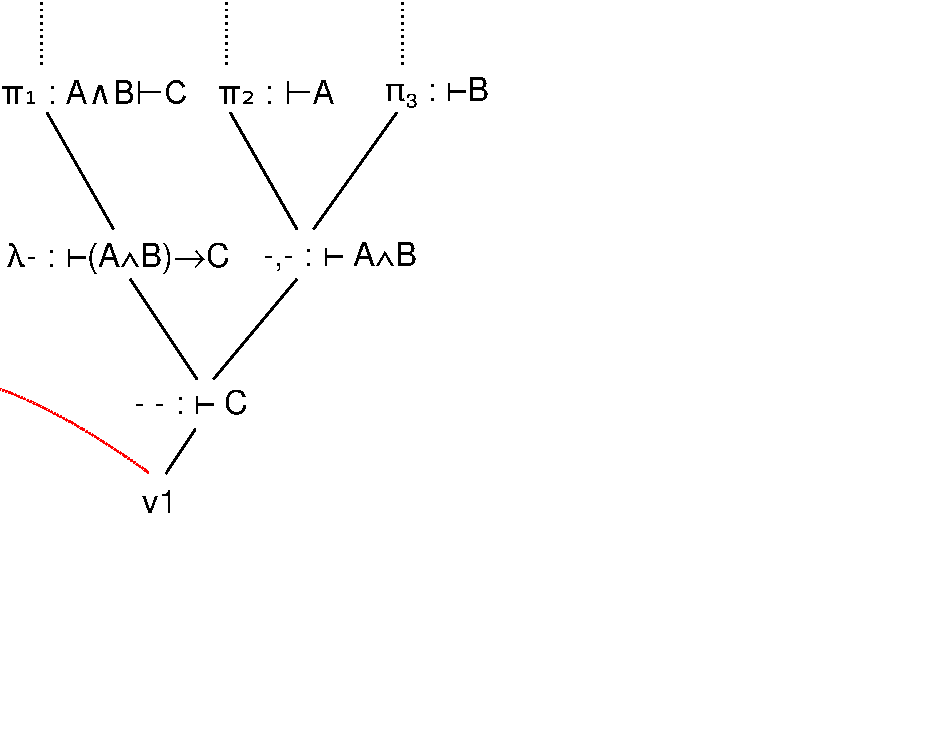
\includegraphics[width=0.85\textwidth]{images/gasp1.pdf}}%
    \only<+>{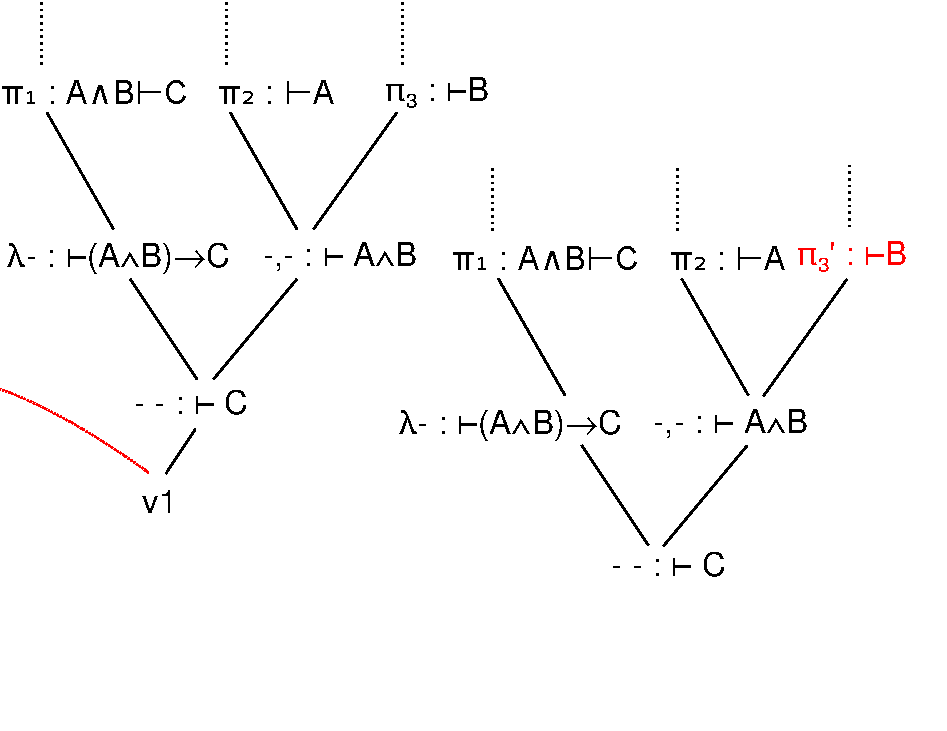
\includegraphics[width=0.85\textwidth]{images/gasp2.pdf}}%
    \only<+>{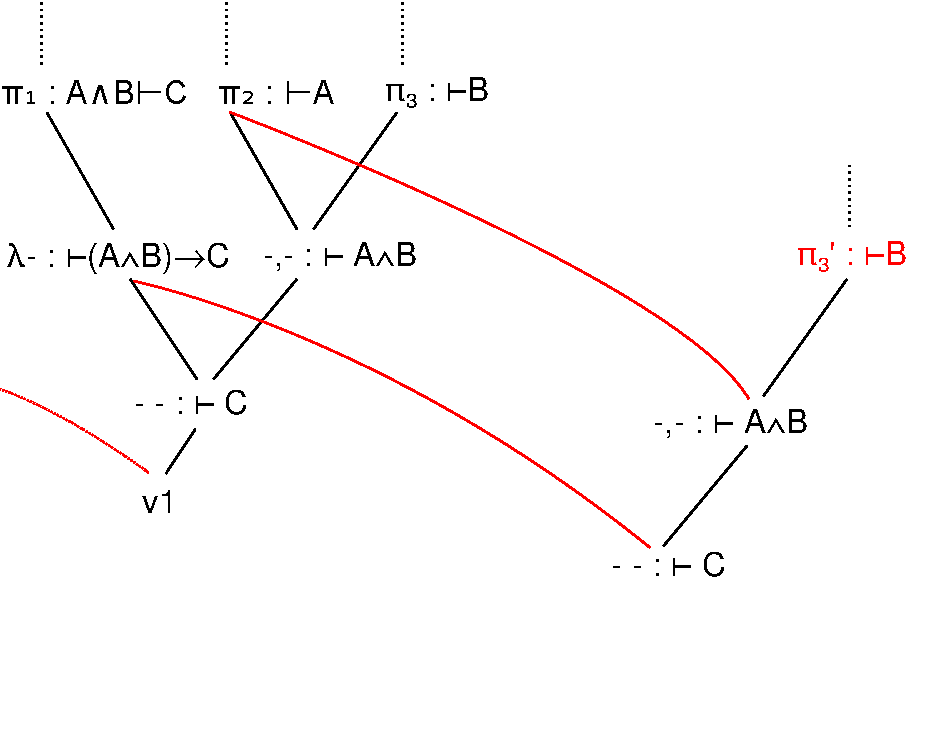
\includegraphics[width=0.85\textwidth]{images/gasp3.pdf}}%
    \only<+>{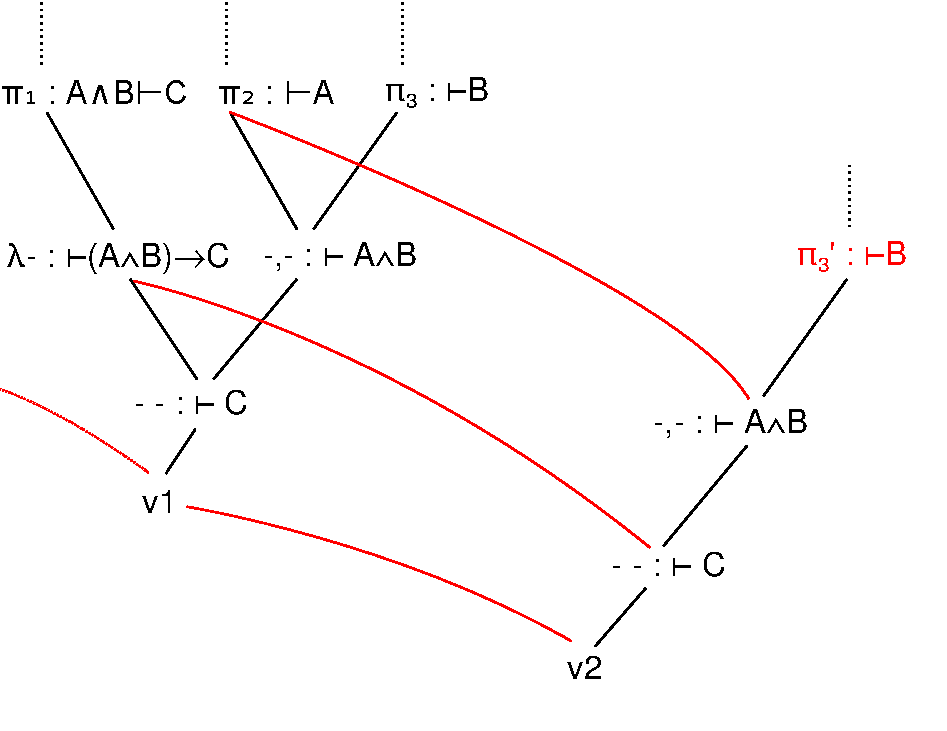
\includegraphics[width=0.85\textwidth]{images/gasp4.pdf}}%
    \only<+>{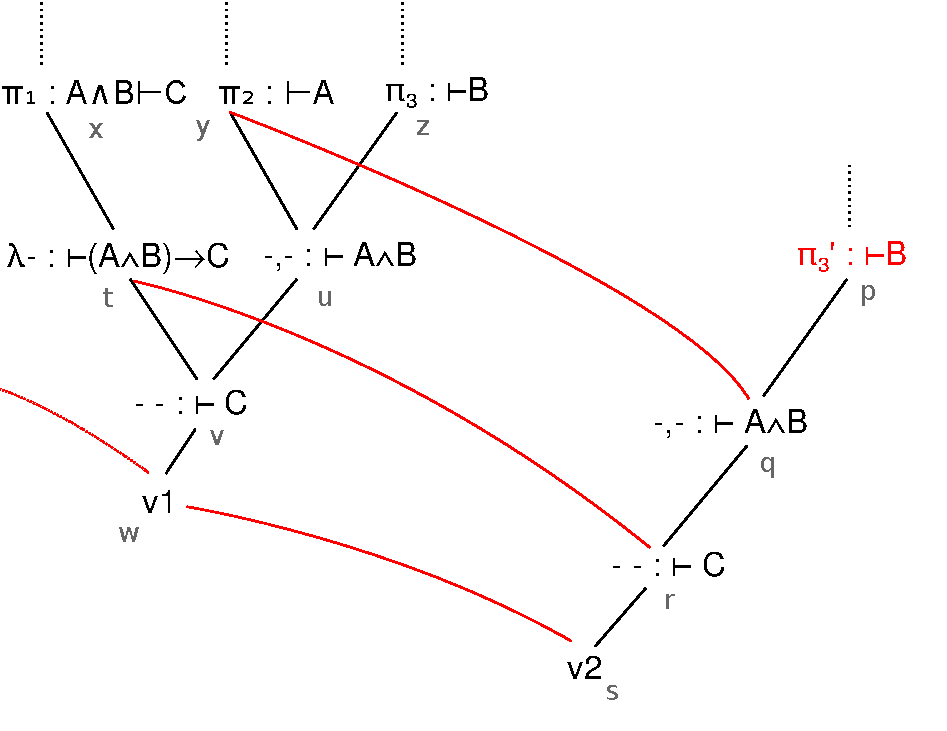
\includegraphics[width=0.85\textwidth]{images/gasp5.pdf}}%
  \end{center}

  \begin{onlyenv}<+->
    \small
    \begin{overlayarea}{0pt}{\textheight}
      \begin{align*}
        x &= \ldots\ : A\wedge B\vdash C \\
        y &= \ldots\ :\ \vdash A \\
        z &= \ldots\ :\ \vdash B \\
        t &= \lam a {A\wedge B} x :\ \vdash A\wedge B\to C \\
        u &= (y, z) :\ \vdash A\wedge B \\
        v &= \app t u :\ \vdash C \\
        w &= \mathsf{Commit}(v,w1) : \mathsf{Version} \only<7>{
          \alert{\qquad,\quad w} }
        \only<8-9>{ \\
          p &=\ldots\ :\ \vdash B \\
          q &= (y, p) :\ \vdash A \wedge B \\
          r &= \app t q :\ \vdash C \\
          s &= \mathsf{Commit}(r,w) : \mathsf{Version} \only<9>{
            \alert{\qquad,\quad s} } }
      \end{align*}
    \end{overlayarea}
  \end{onlyenv}
\end{frame}

\begin{frame}{A data-oriented notion of delta}
  \begin{itemize}
  \item<+-> A delta is a term $t$ with \emph{variables} \alert{$\mv, \mmv
      $}, defined in the repository
  \item<+-> A repository $\mr$ is a \emph{flattened}, \emph{annotated} term with
    a \emph{head}
  \item<+-> Incrementality by \emph{sharing} common subterms
    \begin{center}
      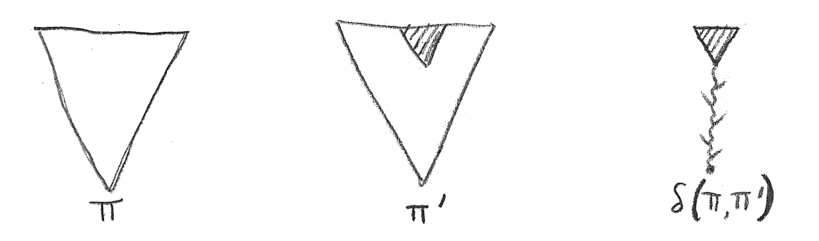
\includegraphics[width=0.90\textwidth]{images/delta.png}
    \end{center}
  \end{itemize}
  \begin{block}{Invariants}<4->
    \begin{itemize}
    \item $\mr$ forms a DAG
    \item Annotations are valid \emph{wrt.} proof rules
    \end{itemize}
  \end{block}
\end{frame}

\begin{frame}{Higher-order notion of delta}
  \only<1>{
    \begin{block}{Problem}
      Proofs are higher-order objects by nature:
      \begin{example}
        \begin{center}
          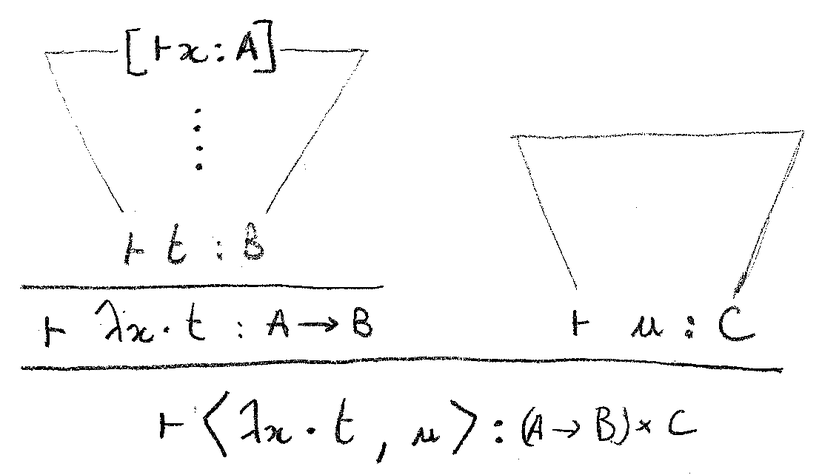
\includegraphics[width=0.60\textwidth]{images/ho-proof.png}
        \end{center}
      \end{example}
      We can't allow sharing in \alert{$\vdash t : B$} without instantiating
      \alert{$\vdash x: A$} (scope escape)
    \end{block}
  }
  \only<2>{
    \begin{block}{Solutions}
      \begin{itemize}
      \item ``first-orderize'' your logic (de Bruijn indices, $\Gamma$ is
        a list\ldots)
        \begin{enumerate}
        \item[\itplus] we're done
        \item[\itminus] weakening, permutation, substitution etc. become
          explicit operations
        \item[\itminus] delta application possibly has to rewrite
          the repository (lift)
          \item[\itminus] dull dull dull\ldots
        \end{enumerate}
        \vspace{1em}
      \item ``let \emph{meta} handle it'' (the delta language)
        \begin{enumerate}
        \item[\itplus] known technique (HOAS)
        \item[\itplus] implicit environments = weakening,
          permutation, substitution for free
        \item[\itminus] have to add an instantiation operator
        \end{enumerate}
      \end{itemize}
    \end{block}
  }
  \only<3>{
    \begin{block}{Solution}
      \begin{center}
        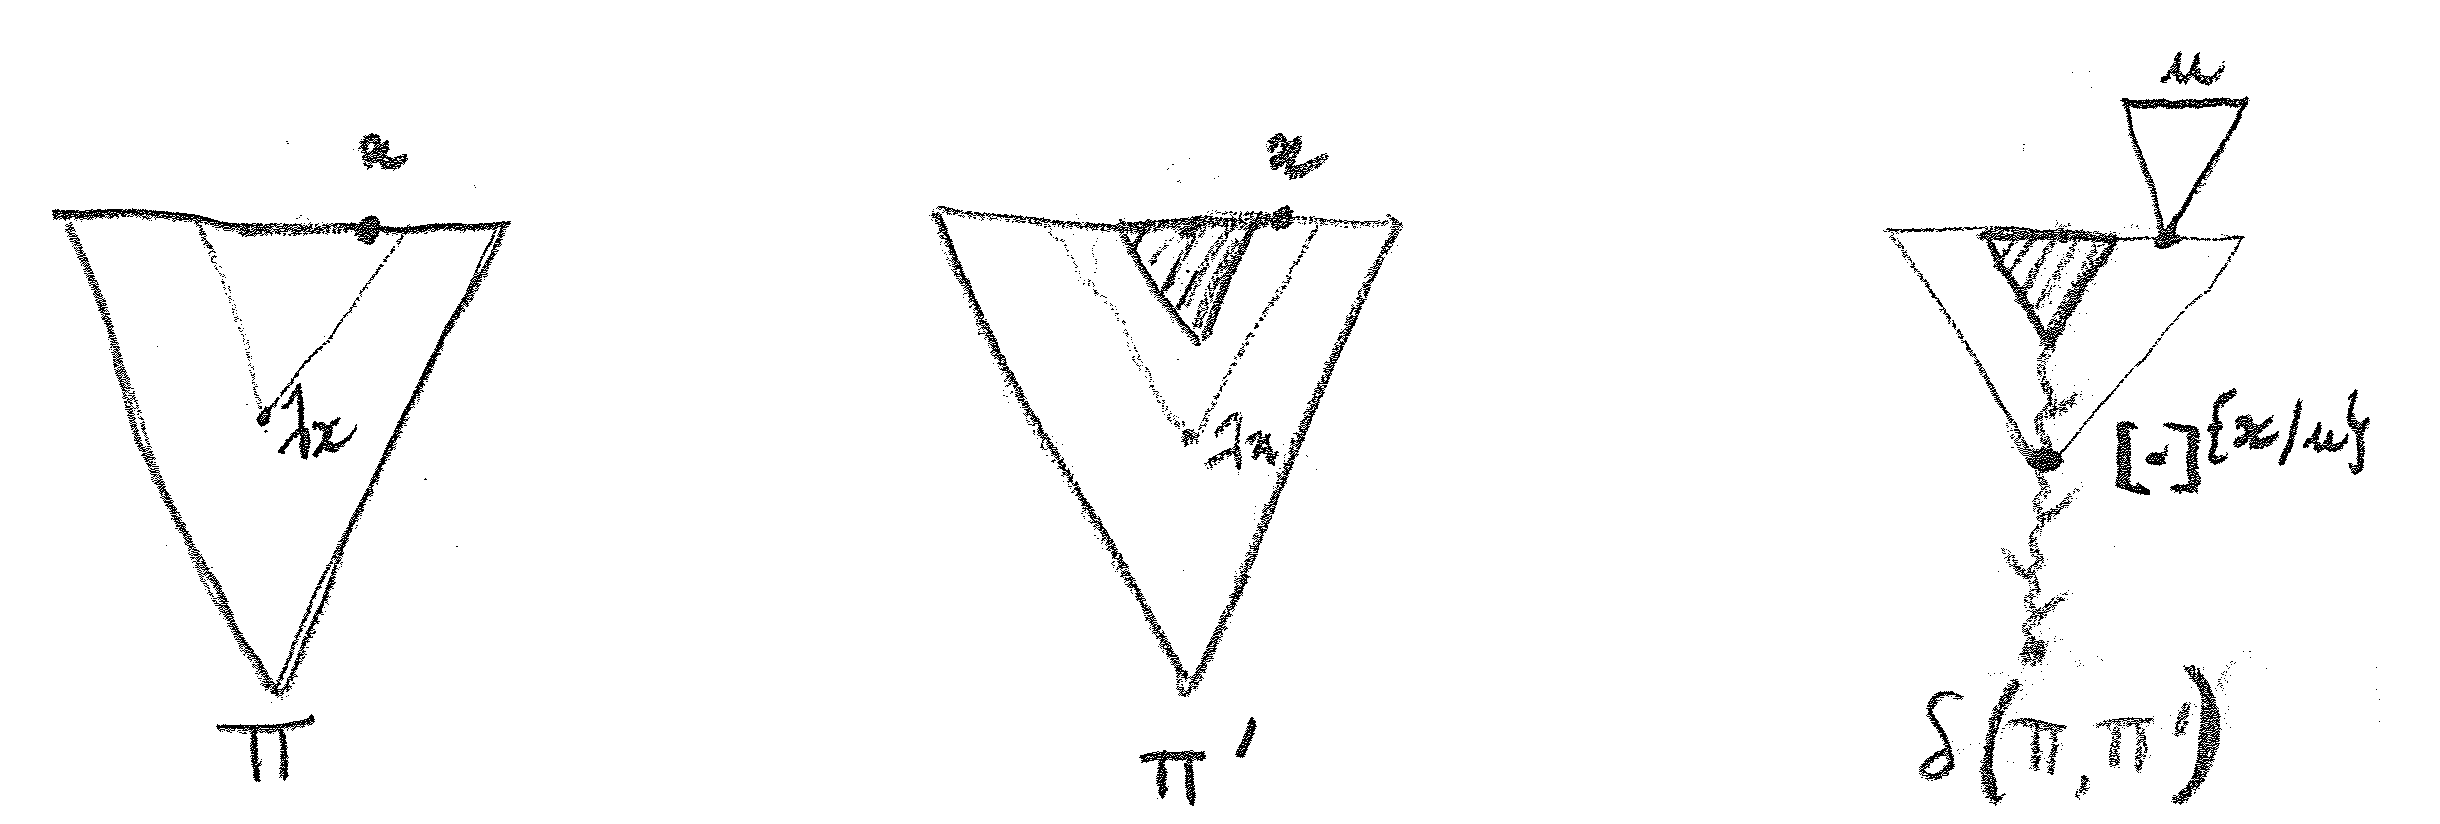
\includegraphics[width=0.90\textwidth]{images/delta2.png}
      \end{center}
      A delta is a term $t$ with variables $x, y$ and boxes \alert{$\ibox t
      {y.n} u$} to jump over lambdas in the repository
    \end{block}
  }
\end{frame}

\begin{frame}{Towards a metalanguage of proof repository}
  \begin{block}{Repository language}
    \begin{enumerate}
    \item name all proof steps
    \item annote them by their judgement
    \end{enumerate}
  \end{block}
  \begin{block}{Delta language}
    \begin{enumerate}
    \item address sub-proofs (variables)
    \item instantiate lambdas (boxes)
    \item check against $\mr$
    \end{enumerate}
  \end{block}
\end{frame}

\section{A metalanguage of repository}

\subsection{Tools}

\subsubsection{The LF logical framework}

\begin{frame}{\gray{A} logical framework \gray{for incremental type-checking}}
  \begin{onlyenv}<-2>
    LF \cit{Harper et al. 1992} (a.k.a. $\lambda\Pi$) provides a {\bf
      meta-logic} to represent and validate syntax, rules and proofs
    of an \textbf{object language}, by means of a typed
    $\lambda$-calculus.

    \begin{description}
    \item[dependent types] to express object-judgements
    \item[signature] to encode the object language
    \item[higher-order abstract syntax] to easily manipulate hypothesis
    \end{description}
    \pause
    \begin{examples}
      \begin{itemize}
      \item \scriptsize
        $
        \begin{array}{c}
          [x:A]\\
          \vdots\\
          t : B \\\hline
          \ulam x t : A\to B
        \end{array}
        \qquad\leadsto\qquad
        \begin{array}{ll}
          \text{\textsf{is-lam}} :& \prd {A,B}{\mathsf{ty}} \prd t {\mathsf{tm}\to \mathsf{tm}} \\
          & (\prd x {\mathsf{tm}} {\textsf{is}\ x\ A} \to \textsf{is}\ (t\ x)\ B) \to \\
          & \textsf{is}\ (\textsf{lam}\ A\ (\ulam x t\ x))(\textsf{arr}\ A\ B)
        \end{array}
        $
      \item
        $
        \begin{array}{c}
          [x:\nat]\\\hline
          \ulam x x : \nat\to\nat
        \end{array}
        \qquad\leadsto\qquad
        \begin{array}{l}
          \text{\textsf{is-lam}}\ \mathsf{nat}\ \mathsf{nat}\ (\ulam x
          x)\ (\ulam {y z} z) \\ \qquad : \mathsf{is}\ (\mathsf{lam}\
          \mathsf{nat}\ (\ulam x x))\ (\mathsf{arr}\ \mathsf{nat}\
          \mathsf{nat})
        \end{array}
        $
      \end{itemize}
    \end{examples}
  \end{onlyenv}
  \begin{onlyenv}<3>
    \inXLF
    \begin{columns}
      \begin{column}{0.6\textwidth}
        \begin{block}{Syntax}
          \vspace{-2em}
          \begin{align*}
            \mk &\gequal { \prd\mv\mf\mk \gor \type } \\
            \mf &\gequal { \prd\mv\mf\mf \gor \lapp\mcf\ma } \\
            \mo &\gequal { \ulam\mv\mo \gor \lapp\mv\ma \gor \lapp\mco\ma } \\
            \ma &\gequal { \lnil \gor \lcons\mo\ma} \\[0.5em]
            \msi &\gequal { \enil \gor \ebinddecl\msi\mco\mf \gor
              \ebinddecl\msi\mcf\mk }
          \end{align*}
        \end{block}
      \end{column}
      \begin{column}{0.4\textwidth}
        \begin{block}{Judgements}
          \begin{itemize}
          \item $\jindex\msi\me\mk$
          \item $\jindex\msi\me\mf$
          \item $\jindex\msi\me {\typ\mo\mf}$
          \item $\jindex\msi{\pair\me\mf} {\typ\ma\mf}$
          \item $\vdash \msi$
          \end{itemize}
        \end{block}
      \end{column}
    \end{columns}
        $$
        \infer{
          \jxlft\Gamma\mo\mf
          \and
          \jxlfa\Gamma{\hsubst\mmf\mv\mo}\ma\mmf
        }{
          \jxlfa\Gamma{\prd\mv\mf\mmf}{\lcons\mo\ma}\mmmf
        }
        $$
    \begin{block}{Remarks}
      \begin{itemize}
      \item the {spine-form}, \alert{canonical} flavor ($\beta$ and
        $\eta$-long normal)
      \item substitution is \alert{hereditary} (\emph{i.e.}
        cut-admissibility / big-step reduction)
      \end{itemize}
    \end{block}
  \end{onlyenv}
\end{frame}

\subsubsection{Monadic LF}

\begin{frame}{Naming of proof steps}
  \begin{onlyenv}<1-2>
    \begin{block}{Remark}
      In LF, proof step = term application spine

      \textcolor{green!50!black}{Example} $ \text{\textsf{is-lam}}\
      \mathsf{nat}\ \mathsf{nat}\ (\ulam x x)\ (\ulam {y z} z) $
    \end{block}
    \pause
    \begin{block}{Monadic Normal Form (\textsf{MNF})}
      Program transformation, IR for FP compilers

      \textbf{Goal:} sequentialize all computations by naming them
      (\textsf{let}s)
      \[
      \inXLF
      \begin{array}{ll}
        \mo &\gequal \ulam\mv\mo \gor \lapp\mo\ma \gor \mv \\
        \ma &\gequal \lnil \gor \lcons\mo\ma \\
      \end{array}
      \ \Longrightarrow\ \inXLFa
      \begin{array}{ll}
        \mo &\gequal \ret\mval \gor \letb\mv{\lapp\mval\ma}\mo \gor \lapp\mval\ma \\
        \ma &\gequal \lnil \gor \lcons\mval\ma \\
        \mval &\gequal \mv \gor \ulam\mv\mo
      \end{array}
      \]
      \begin{examples}
        \begin{itemize}
        \item $\inXLFa \lapp f {\lapp g {\lsing x}} \quad\notin\quad
          \mathsf{MNF}$
        \item $\ulam x \lapp f {\lsing{\lapp g {\lcons{\ulam y
                  y}{\lsing x}}}} \quad\Longrightarrow\quad
          \ret{(\ulam x \letb a {{\lapp g {\lcons{\ulam y y}{\lsing
                    x}}}} \lapp f {\lsing a})} $
        \end{itemize}
      \end{examples}
    \end{block}
  \end{onlyenv}
  \begin{onlyenv}<3->
    \begin{block}{Positionality inefficiency}
      Order of \textsf{let}s is irrelevant, we just want
      non-cyclicity and fast access.
      \inXLFa
      \[
      \begin{array}{l}
        \letb x \ldots \\
        \quad \letb y \ldots \\
        \quad\quad\letb z \ldots \\
        \quad\quad\quad\vdots \\
        \quad\quad\quad\quad\lapp\mval\ma
      \end{array}
      \pause
      \quad\Longrightarrow\quad
      \sapply{\left(
        \begin{array}{l}
          x=\ldots \\
          y=\ldots \\
          z=\ldots \\
          \vdots
        \end{array}
      \right)}
      {\lapp\mval\ma}
      \]
    \end{block}
    \pause
    \vspace{-2em}
    \begin{block}{Non-positional monadic calculus}
      \inXLFa
      \begin{overlayarea}\textwidth{5em}
        \vspace{-1em}
        \begin{align*}
          \mo &\gequal \ret\mval \gor \alt<4>
          {\letb\mv{\lapp\mval\ma}\mo \gor \lapp\mval\ma}
          {\alert{\sapply\ms{\lapp\mval\ma}}} \\
          \ma &\gequal \lnil \gor \lcons\mval\ma \\
          \mval &\gequal \mv \gor \ulam\mv\mo
          \alt<4>{}{\\
            \alt<5>
            {\alert\ms &\alert{\gequal \snil \gor \scons\ms\mv{\lapp\mval\ma}} }
            {\ \alert\ms\ &\alert{:\ \mv\mapsto{\lapp\mval\ma}}}
          }
        \end{align*}
        \pause
      \end{overlayarea}
    \end{block}
  \end{onlyenv}
  \pause
\end{frame}

\begin{frame}{Monadic LF}
  \inXLF
  \begin{align*}
    \mk &\gequal \prd\mv\mf\mk \gor \type \\
    \mf &\gequal \prd\mv\mf\mf \gor \sapply\ms{\lapp\mcf\ma} \\
    \mo &\gequal \alt<-1>{\ret\mval\gor}{\alt<-2>{\alert{\ret\mval
          \gor}}{}} \sapply\ms{\alt<-1>{\lapp\mval\ma}{\alt<-2>{\alert{\lapp\mval\ma}}{\mval}}} \\
    \mh &\gequal \mv \gor \mco \\
    \ma &\gequal \lnil \gor \lcons\mval\ma \\
    \mval &\gequal \mco \gor \mv \gor \ulam\mv\mo \\
    \ms\ &\ :\ \mv\mapsto{\lapp\mh\ma} \\
    \msi &\gequal { \enil \gor \ebinddecl\msi\mco\mf \gor
      \ebinddecl\msi\mcf\mk }
  \end{align*}
  \pause\pause\pause
 \begin{definition}
    $$ \fflatten\cdot \quad:\quad \text{LF} \to \text{monadic LF} $$
    One-pass, direct style version of \cit{Danvy 2003}
 \end{definition}
\end{frame}

\subsection{Typing by annotating}

\begin{frame}{\alt<-2>{Type annotation}{The repository language}}
  \begin{block}{Remark}
    In LF, judgement annotation = type annotation

    \begin{example}
      $
      \begin{array}{l}
        \text{\textsf{is-lam}}\ \mathsf{nat}\ \mathsf{nat}\ (\ulam x
        x)\ (\ulam {y z} z) \\ \qquad : \mathsf{is}\ (\mathsf{lam}\
        \mathsf{nat}\ (\ulam x x))\ (\mathsf{arr}\ \mathsf{nat}\
        \mathsf{nat})
      \end{array}
      $
    \end{example}
  \end{block}
  \pause
  \alt<-2>\inXLF\inXLFa
  \begin{align*}
    \mk &\gequal \prd\mv\mf\mk \gor \type \\
    \mf &\gequal \prd\mv\mf\mf \gor \sapply\ms{\lapp\mcf\ma} \\
    \alt<2>\mo{\alert\mr} &\gequal
    \sapply\ms{\typ\mval{\alert{\lapp\mcf\ma}}} &&
      \uncover<4->{\text{$\longleftarrow$ $\ms$ DAG, binds in $\mval$ and
          $\ma$}} \\
    \mh &\gequal \mv \gor \mcf \\
    \ma &\gequal \lnil \gor \lcons\mval\ma \\
    \mval &\gequal \mco \gor \mv \gor \lam\mv{\alert\mf}{\alt<2>\mo{\alert\mr}} \\
    \ms\ &\ :\ \mv\mapsto{\laapp\mh\ma{\alert{\lapp\mcf\ma}}} &&
      \uncover<5->{\text{$\longleftarrow$ named implementation}} \\
    \msi &\gequal { \enil \gor \ebinddecl\msi\mco\mf \gor
      \ebinddecl\msi\mcf\mk }
  \end{align*}
\end{frame}

\begin{frame}{The delta language}
  \inXLF
  \begin{columns}
    \begin{column}{0.6\textwidth}
      \begin{block}{Syntax} \vspace{-2em}
        \begin{align*}
          \mk &\gequal { \prd\mv\mf\mk \gor \type } \\
          \mf &\gequal { \prd\mv\mf\mf \gor \lapp\mcf\ma } \\
          \mo &\gequal { \ulam\mv\mo \gor \lapp\mv\ma \gor \lapp\mco\ma
            \gor \alert{\ibox\mo{\mv.n}\mo}
          } \\
        \ma &\gequal { \lnil \gor \lcons\mo\ma} \\[0.5em]
          \msi &\gequal { \enil \gor \ebinddecl\msi\mco\mf \gor
            \ebinddecl\msi\mcf\mk }
        \end{align*}
      \end{block}
    \end{column}
    \begin{column}{0.4\textwidth}
      \begin{block}{Judgements}
        \begin{itemize}
        \item $\jannK{\alert\mr}\me\mk{\alert\mk}$
        \item $\jannA{\alert\mr}\me\mf{\alert\mf}$
        \item $\jannt{\alert\mr}\me\mo\mf{\alert\mo}$
        \item $\jannl{\alert\mr}\me\mf\ma{\alert\ma}\mf$
        \item $\jannsi\msi{\alert\msi}$
        \end{itemize}
      \end{block}
    \end{column}
  \end{columns}
  \begin{block}{Informally}
    \begin{itemize}
    \item $\jindex\msi{\pair\mr\me}\mv\To\mr$ {\footnotesize
        means}\\ “I am what $\mv$ stands for, in $\me$ or in $\mr$ (and produce $\mr$)”.
    \item $\jindex\msi{\pair\mr\me}{\ibox\mo{\mmv.n}\mmo}\To\mmr$
      {\footnotesize means}\\ “Variable $\mmv$ has the form
      $\lapp\mco{\mmmo_1\ldots\mmmo_{n-1}(\ulam x \mmmr)\ldots}$ in $\mr$. Make all
      variables in $\mmmr$ in scope for $\mo$, taking
      $\mmo$ for $\mv$.

      In this new scope, $\mo$ will produce $\mmr$”
    \end{itemize}
  \end{block}
\end{frame}

\subsection{The typing/committing process}

\subsubsection{What does it do?}

\begin{frame}{The typing/committing process}
  \inXLF
  {\Large
  \[
  \jannt\mr\me\mo\mf\mo
  \]}
  \begin{block}{What does it do?}
    \begin{itemize}
    \item puts $\mo$ in non-pos. \textsf{MNF} ($O(\mo)$)
    \item type-checks $\mo$ \emph{wrt.} $\inXLFa\mr$ and
    \item returns $\inXLFa\mo$ \emph{i.e.} $\inXLF\mo$ annotated with types ($O(\mo)$)
    \end{itemize}
  \end{block}
\end{frame}

\begin{frame}{Typing by annotating}
  \textbf{partial translation} : monadic LF $\to$ annotated monadic LF
  \inXLFa
  \Large
  \begin{overlayarea}\textwidth{10em}
    \only<+>{
      $$
      \infer[VLam]{ \jannt\mr{\ebinddecl\me\mv\mf}\mo\mmf\mo }{
        \jannv\mr\me{\ulam\mv\mo}{\prd\mv\mf\mmf}{\lam\mv\mf\mo} }
      $$
    }
    \only<+>{
      $$
      \infer[HVar]{ \elookdecl\me\mv\mf \and\text{or}\and
        \elookdecl\ms\mv\mf }{ \jannh{(\sapply\ms\mval)}\me\mv\mf }
      $$
    }
    \only<+>{
      $$
      \infer[LCons]{ \jannv\mr\me\mval\mf\mval \and
        \jannl\mr\me{\hsubst\mmf\mv\mval}\ma\ma{\lapp\mcf\ma} }{
        \jannl\mr\me{\prd\mv\mf\mmf}{\lcons\mval\ma}{\lcons\mval\ma}{\lapp\mcf\ma}
      }
      $$
    } \only<+>{
      $$
      \infer[OBox]{ \mr|_p = \lam\mv\mmf\mmr \and
        \jannt\mr\me\mmo\mmf{(\sapply\ms{\typ\mh{\lapp\mcf\ma}})}
        \\
        \jannt{\mmr\cup\scons\ms\mv{\typ\mh{\lapp\mcf\ma}}}\me\mo\mf\mo }{
        \jannt\mr\me{\ibox\mo p\mmo}\mf\mo }
      $$
    }
    \normalsize
    \only<+>{
      \begin{align*}
        \sz{(\prd\mv\mf\mmf)} &= \prd\mv{\sz\mf}{\sz\mmf} \\
        \sz{(\sapply\ms{\lapp\mcf\ma})} &=
        \sapply{\sz\ms}{\lapp\mcf{\sz\ma}} \\[1em]
        \sz{(\scons\ms\mmv{\lapp\mv\ma:\lapp\mcf\mma})} &=
        \scons{(\sz\ms)}\mmv{\lapp\mv{\sz\ma}:\lapp\mcf{\sz\mma}} \\
        \sz{(\scons\ms\mmv{\lapp\mmmv\ma:\lapp\mcf\mma})} &=
        \fred\mmv\ms\mval\ma \\[1em]
        \fred\mmv\ms{\mh:\lapp\mcf\ma}\lnil &=
        \scons\ms\mmv{\mh:\lapp\mcf\ma} \\
        \fred\mmv\ms{\lam\mv\mf\mo}{(\lcons\mval\ma)} &=
        \fred\mmv{\ms\cup\mms}\mmval\ma
        \qquad\text{if}\quad
        \hsubst\mo\mv\mval = (\sapply\mms\mmval) \\
        &\vdots
      \end{align*}
    }
  \end{overlayarea}
\end{frame}

\begin{frame}{Properties of the translation}
  Work in progress\ldots
  \begin{theorem}[Soundness]
    if $\jxlft\me\mo\mf$ then $\jannsi{\fflatten\me}\me$ and $\jannA{(\sapply\snil\_)}\me{\fflatten\mf}\mf$ and
    $\jannt{(\sapply\snil\_)}\me{\fflatten\mo}\mf\mo$
  \end{theorem}
  \begin{definition}[Checkout]
    Let $\fcheckout\cdot$ be the back-translation
    function of a repository into an LF term.
  \end{definition}
  \begin{theorem}[Completeness]
    if $\jannt{(\sapply\snil\_)}\me{\fflatten\mo}\mf\mo$ then $\jxlft{\fcheckout\me}{\fcheckout\mo}{\fcheckout\mf}$
  \end{theorem}
  \begin{theorem}[Substitution]
    If $\jannt\mr\me\mmo\mmf{(\sapply\ms{\mmv:\mmf})}$ and
    $\jxlft{\econs{\fcheckout\me}{x:\mmf}{\fcheckout\mme}}\mo\mf$ then
    $\jannt{(\sapply\ms{\mmv:\mmf})}{\me{\repl\mme\mv\mmv}}{\repl\mo\mv\mmv}{\repl\mmf\mv\mmv}\mmr$
  \end{theorem}
\end{frame}

\subsubsection{Example}

\begin{frame}{Example}
  \underline{Signature}
  \begin{align*}
    A&\ B\ C\ D : * \\
    a &: (D\to B)\to C\to A     & b&\ b' : C\to B \\
    c &: D\to C                 & d &: D
  \end{align*}
  \underline{Terms}
  \small
  \begin{align*}
    t_1\ &=\quad
    \lapp a {\lcons{\ulam x \lapp b {\lapp c x}}{\lapp c d}} \\
    \mr_1\ &=\quad
    \sent v {\lapp c d : C} \\
    &\ \qquad\sent u {\lapp a {\lcons{\lam x D
          \sent w {\lapp c x : C}\sent {w'} {\lapp b w : B}\vdash w' :
          B}{v}} : A} \\
    &\ \qquad\qquad\vdash u : A\\
    t_2 \ &=\quad
    \lapp a {\ulam y {\ibox {\lapp{b'} w} 1 x y}} \\
    \mr_2\ &=\quad
    \sent v {\lapp c d : C} \\
    &\ \qquad\sent u {\lapp a {\lcons{\lam y D
          \sent x y \sent w {\lapp c x : C} \sent {w'} {\lapp b w : B}\vdash w' :
          B}{v}} : A} \\
    &\qquad\qquad \vdash u : A
  \end{align*}
\end{frame}

\subsubsection{Regaining version management}

\begin{frame}{Regaining version management}
  \inXLF
  Just add to the signature $\msi$:
  \begin{align*}
    \mathsf{Version} &: \type \\
    \mathsf{Commit0} &: \mathsf{Version} \\
    \mathsf{Commit} &:
    \prd t {\mathsf{tm}}{\lapp{\mathsf{is}}{\lcons{t}{\mathsf{unit}}} \to
    \mathsf{Version} \to \mathsf{Version}}
  \end{align*}
  \vspace{-2em}
  \begin{block}{Commit $t$}
    \vspace{-1em}
    \[ \text{if} \qquad
    \mr = \sapply\ms{v : \mathsf{Version}} \qquad\text{and}\qquad
    \mr,\enil\vdash_\msi t : \lapp{\mathsf{is}}{\lcons p
      {\mathsf{unit}}}\To(\mms\vdash k)
    \]
    then
    \[\scons\mms\mv{\lapp{\mathsf{Commit}}{\lcons p {\lcons k v}}}\vdash x :
    \mathsf{Version}\]
    is the new repository
  \end{block}
\end{frame}

\begin{frame}{Further work}
  \begin{itemize}
  \item metatheory of annotated monadic LF
  \item from terms to derivations (\textsf{ti})
  \item \textsf{diff} on terms
  \item mimick other operations from VCS (\textsf{Merge})
  \end{itemize}
  \vspace{2em}
  \pause
  \begin{center}
    \Large\em Thank you!
  \end{center}
\end{frame}

\end{document}

%%% Local Variables: 
%%% mode: latex
%%% TeX-master: t
%%% End: 
